%% Supplementary Information: thematic sections; figures numbered in order of appearance.
%% Structure documented in documentation/SUPPLEMENTARY_STRUCTURE.md

\clearpage
\setcounter{figure}{0}
\renewcommand{\thefigure}{S\arabic{figure}}
\setcounter{table}{0}
\renewcommand{\thetable}{S\arabic{table}}

\section*{Supplementary Information}

\noindent This supplement follows the main paper: theoretical derivations, then the idealised probit check, then the sports KPI analysis. Figures are numbered in order of appearance (S1--S3). File names on disk retain their generator tags and need not match the printed S-number.

\medskip
\noindent\begin{tabular}{@{}p{0.22\linewidth}p{0.34\linewidth}p{0.38\linewidth}@{}}
  \toprule
  \textbf{SI block} & \textbf{Main paper} & \textbf{Contents} \\
  \midrule
  \S1 Theory & Theory; Intro.\ (Pitman) & Algebra; $\tau=\tfrac12\log\kappa$; Pitman ARE \\
  \S2 Probit validation & Methods Tier~1; Results & Spec.; Figs~S1--S2 \\
  \S3 Empirical analysis & Methods; Results; Discussion & Fig.~S3; Table~S1; QC \\
  \bottomrule
\end{tabular}

\clearpage

% ---------------------------------------------------------------------------
\refstepcounter{sisection}
\section*{SI Section \thesisection: Theoretical Derivations}
\label{sec:si_maths}

\noindent This section supports the theoretical framework (\cref{sec:theory}). The main text states the integral for $I(X;Y)$ (\cref{eq:mi_closed}) and the four-cell partition. This section records the omitted algebra. The sports cloud is \cref{fig:pef_landscape}.

%% SI Section 1 (mathematical derivations). Input from sections/supplementary.tex.
\label{sec:si_note_s3}
\label{sec:appendix}

\noindent The algebraic derivation of the PEF formula (\cref{eq:pef}) from the variance of correlated differences, together with its reduction to Fisher's classical case at $\kappa=1$, is given in full in \cref{sec:theory}. This section records a log-ratio remapping of $\kappa$, the information-content integral and its Jensen bound, and the Pitman asymptotic relative efficiency argument.

\subsection*{Log-ratio coordinate for the variance ratio}
\label{sec:si_tau}

The variance ratio $\kappa=\sigma_{\mathrm{B}}^{2}/\sigma_{\mathrm{A}}^{2}$ is multiplicative. An additive remapping that places equal variances at the origin is the log standard-deviation ratio
\begin{equation}
  \tau \;=\; \log\frac{\sigma_{\mathrm{B}}}{\sigma_{\mathrm{A}}} \;=\; \tfrac12\log\kappa.
  \label{eq:tau_remap}
\end{equation}
The map $\kappa\mapsto\tau$ is strictly increasing on $(0,\infty)$, and $\tau=0$ if and only if $\kappa=1$. Interchanging the labels of A and B sends $\kappa\mapsto 1/\kappa$ and therefore $\tau\mapsto-\tau$. The four quadrants of the $(\kappa,\rho)$ plane then occupy the four open quadrants of the $(\rho,\tau)$ plane. The main text stays in $(\kappa,\rho)$.

\subsection*{Information Content Derivation}
\label{sec:si_maths_detail}

\paragraph*{Setup}

Under (A1), $X\sim\mathcal{N}\bigl(\delta,\sigma^{2}_{\mathrm{A}}(1+\kappa-2\sqrt{\kappa}\,\rho)\bigr)$ with $\delta=\mu_{\mathrm{A}}-\mu_{\mathrm{B}}$. Under (A2), $\mathbb{P}(Y=1\mid X=x)=\Phi(x/\sqrt{\Var(X)})$. Let $U\sim\mathcal{N}(0,1)$ and $d_{\mathrm{rel}}=|\delta|/\sqrt{\Var(X)}$ as in \cref{eq:drel}. Then $X/\sqrt{\Var(X)}$ has the same distribution as $d_{\mathrm{rel}}+U$ or as $-(d_{\mathrm{rel}}+U)$, and binary entropy satisfies $h(p)=h(1-p)$, so the sign of $\delta$ does not change $I(X;Y)$.

\paragraph*{Marginal entropy}

The marginal success probability is the Gaussian identity $\mathbb{E}[\Phi(d_{\mathrm{rel}}+U)]=\Phi(d_{\mathrm{rel}}/\sqrt{2})$. Therefore
\begin{equation*}
  H(Y) = h\!\left(\Phi\!\left(\frac{d_{\mathrm{rel}}}{\sqrt{2}}\right)\right).
\end{equation*}
This equals $1$ bit only at $d_{\mathrm{rel}}=0$.

\paragraph*{Conditional entropy and the integral}

\begin{equation*}
  H(Y\mid X) = \mathbb{E}\bigl[h\bigl(\Phi(d_{\mathrm{rel}}+U)\bigr)\bigr]
  = \int_{-\infty}^{\infty} h\bigl(\Phi(d_{\mathrm{rel}}+u)\bigr)\,\phi(u)\,du,
\end{equation*}
where $\phi$ is the standard normal density. The reported values of \cref{eq:mi_closed} are this integral minus nothing further: $I(X;Y)=H(Y)-H(Y\mid X)$, computed by adaptive quadrature on $[-10,10]$. From \cref{eq:pef}, $\Var(X)=\sigma^{2}_{\mathrm{A}}(1+\kappa)/\eta$, which is the route from $(\kappa,\rho)$ to $d_{\mathrm{rel}}$ in \cref{eq:drel}.

\paragraph*{Jensen bound}

Let $p(x)=\Phi(x/\sqrt{\Var(X)})$ and $m(x)=\min(p(x),1-p(x))\in[0,1/2]$. Then $h(p(x))=h(m(x))$, and $h$ is concave on $[0,1/2]$, so Jensen's inequality gives $H(Y\mid X)=\mathbb{E}[h(m(X))]\le h(\mathbb{E}[m(X)])=h(P_{e})$. Rearrangement is \cref{eq:mi_bound}. The Bayes error here is $P_{e}=1-\mathbb{E}[\Phi(|d_{\mathrm{rel}}+U|)]$, the error of the sign rule, not $\Phi(-d_{\mathrm{rel}}/2)$.

The expression $1-h(\Phi(d_{\mathrm{rel}}/2))$ assumes $H(Y)=1$ and a different error rate. It is not a lower bound under (A1)--(A2), and it is not used for any reported information value.

\subsection*{Connection to Pitman Asymptotic Relative Efficiency}
\label{sec:pitman}

This section establishes that, under bivariate normality and equal group sizes, the PEF equals the Pitman asymptotic relative efficiency (ARE) of the paired $t$-test relative to the independent two-sample $t$-test. We state this as a proposition, give a self-contained proof, verify the classical reduction, and record the qualifications that bound the result.

\paragraph*{Proposition}

\noindent\textbf{Proposition (PEF as Pitman ARE).} \emph{Under Assumption~(A1) and equal allocation ($n$ observations per group), the Pitman ARE of the paired $t$-test relative to the independent two-sample $t$-test equals}
\begin{equation}
  \mathrm{ARE}_{\mathrm{paired/indep}} = \frac{1+\kappa}{1+\kappa-2\sqrt{\kappa}\,\rho} = \eta.
  \label{eq:are_pef}
\end{equation}

\paragraph*{Proof}

Let $N=2n$ be the total number of observations available. Fix $\mu_{\mathrm{A}}-\mu_{\mathrm{B}}=\delta>0$ and let $n\to\infty$. We compare the noncentrality parameters of the two tests at the same total sample size.

\medskip
\noindent\textbf{Step 1: Paired test.} With $n$ matched pairs, differences $D_i=X_{\mathrm{A},i}-X_{\mathrm{B},i}\sim\mathcal{N}(\delta,\sigma^{2}_{\mathrm{A}}(1+\kappa-2\sqrt{\kappa}\,\rho))$ are i.i.d.\ under (A1). The noncentrality parameter of $T_p=\bar{D}/\sqrt{s^{2}_{D}/n}$ is
\begin{equation}
  \lambda_{p}(n) = \frac{\delta\sqrt{n}}{\sigma_{\mathrm{A}}\sqrt{1+\kappa-2\sqrt{\kappa}\,\rho}}.
  \label{eq:ncp_paired}
\end{equation}

\noindent\textbf{Step 2: Independent two-sample test.} With $n$ independent observations per group (total $N=2n$, equal allocation), the noncentrality parameter of the Welch $t$-test $T_u=(\bar{X}_{\mathrm{A}}-\bar{X}_{\mathrm{B}})/\sqrt{s^{2}_{\mathrm{A}}/n+s^{2}_{\mathrm{B}}/n}$ is
\begin{equation}
  \lambda_{u}(n) = \frac{\delta\sqrt{n}}{\sigma_{\mathrm{A}}\sqrt{1+\kappa}}.
  \label{eq:ncp_unpaired}
\end{equation}

\noindent\textbf{Step 3: ARE.} Both tests use the same total sample $N=2n$. The Pitman ARE is the limiting ratio of sample sizes required for equal power at fixed significance and effect size, which equals the ratio of squared noncentrality parameters per observation \parencite{lehmann1999}:
\begin{equation}
  \mathrm{ARE}_{\mathrm{paired/indep}}
    = \lim_{n\to\infty}\frac{n_{u}^{*}}{n_{p}^{*}}
    = \frac{\lambda_{p}^{2}(n)/n}{\lambda_{u}^{2}(n)/n}
    = \frac{\delta^{2}/\bigl(\sigma^{2}_{\mathrm{A}}(1+\kappa-2\sqrt{\kappa}\,\rho)\bigr)}
           {\delta^{2}/\bigl(\sigma^{2}_{\mathrm{A}}(1+\kappa)\bigr)}
    = \frac{1+\kappa}{1+\kappa-2\sqrt{\kappa}\,\rho}
    = \eta \phantom{00} \qedsymbol{}.
\end{equation}

\paragraph*{Classical Verification}

Setting $\kappa=1$:
\begin{equation*}
  \mathrm{ARE}_{\mathrm{paired/indep}} = \frac{2}{2-2\rho} = \frac{1}{1-\rho},
\end{equation*}
recovering Fisher's classical paired-design efficiency \parencite{fisher1935}. The PEF is therefore the direct generalisation of Fisher's result to unequal variances, expressed in the language of Pitman efficiency.

\paragraph*{Qualifications}

Three conditions bound \cref{eq:are_pef}:

\begin{enumerate}
  \item \textbf{Normality.} Steps~1--2 use the normal noncentrality parameter. Under non-normality, the central limit theorem ensures the limiting noncentrality is still given by \cref{eq:ncp_paired,eq:ncp_unpaired} under finite second moments, so the ARE result is asymptotically robust; however, the small-sample comparison may differ.

  \item \textbf{Equal group allocation.} Step~2 assumes $n_{\mathrm{A}}=n_{\mathrm{B}}=n$. Unequal allocation, including Neyman allocation $n_{\mathrm{A}}/n_{\mathrm{B}}=\sigma_{\mathrm{A}}/\sigma_{\mathrm{B}}$, changes the noncentrality of the independent test and therefore changes the ARE. Equal allocation is the comparison used here, because the paired and unpaired designs are then given the same total sample in the same proportions.

  \item \textbf{Fixed alternative.} The result above uses a fixed $\delta$ and $n\to\infty$. Under local (Pitman) contiguous alternatives $\delta_{n}=c/\sqrt{n}$, the noncentrality parameters remain $O(1)$ and the same ratio $\eta$ is obtained in the limit, so the result is unchanged \parencite{lehmann1999}.
\end{enumerate}

\noindent The PEF formula is distribution-free (\cref{eq:pef}); only the ARE \emph{interpretation} in \cref{eq:are_pef} requires normality. The distribution-free efficiency characterisation (the variance ratio) is the primary result; the Pitman ARE connection provides a classical testing-theory corroboration.


\subsection*{Information content}
\label{sec:si_theory}

\noindent The integral and the Jensen bound are derived below. Cuts of $\eta$ and $I(X;Y)$ at the median empirical $|\hat d_Y|$ and at $\delta/\sigma_{\mathrm{A}}=1$ are \cref{fig:si_iso_eta_I}, in the probit section.

\clearpage

% ---------------------------------------------------------------------------
\refstepcounter{sisection}
\section*{SI Section \thesisection: Idealised Probit Validation}
\label{sec:si_probit}

\noindent This section supports the first validation tier (\cref{sec:methods}): an idealised probit simulation under (A1)--(A2) that evaluates the integral for $I(X;Y)$ (\cref{eq:mi_closed}) and the efficiency--power tension (\cref{sec:eff_power_theory}) before turning to empirical KPIs. Main-text scenario results appear in \cref{sec:results,tab:scenarios}; the specification below is the full model; \cref{fig:si_idealised_stratified,fig:si_iso_eta_I} visualise grid-level and contour-level behaviour cited in \cref{sec:results,sec:signal_strength}.

\subsection*{Idealised Probit Simulation: Model Specification and Validation}
\label{sec:si_note_s2}

\textbf{Purpose.} The first validation tier (\cref{sec:methods}) isolates the PEF--information content relationship (\cref{eq:mi_closed}) from the finite-sample noise, mild non-normality, and team-level clustering present in the empirical KPIs. Data are generated to satisfy (A1)--(A2) exactly. The simulation then checks two claims. First, the integral is tracked by five-fold logistic regression, the same classifier family as the empirical protocol. Pairs are independent by construction, so the simulation does not use team-blocked folds. Second, the efficiency--power tension (\cref{sec:eff_power_theory}) arises as predicted. This is a check of internal consistency under the model's own assumptions, not an independent empirical test. The empirical tiers (\cref{sec:results}) provide the latter.

\textbf{Data-generating process (A1).} For each grid cell $(\kappa,\rho,\delta/\sigma_{\mathrm{A}})$ we draw $n$ independent pairs from the bivariate normal
\begin{equation}
  \begin{pmatrix}X_{\mathrm{A}}\\[2pt] X_{\mathrm{B}}\end{pmatrix}
  \sim \mathcal{N}\!\left(
  \begin{pmatrix}\delta/2\\[2pt] -\delta/2\end{pmatrix},\;
  \sigma_{\mathrm{A}}^{2}
  \begin{pmatrix}1 & \rho\sqrt{\kappa}\\[2pt] \rho\sqrt{\kappa} & \kappa\end{pmatrix}
  \right),
  \label{eq:si_dgp}
\end{equation}
with $\sigma_{\mathrm{A}}=1$. This parameterisation fixes $\Var(X_{\mathrm{A}})=\sigma_{\mathrm{A}}^{2}$, $\Var(X_{\mathrm{B}})=\kappa\sigma_{\mathrm{A}}^{2}$, and $\Corr(X_{\mathrm{A}},X_{\mathrm{B}})=\rho$, so the variance ratio and correlation match their targets by construction. The relative feature $X=X_{\mathrm{A}}-X_{\mathrm{B}}$ then has mean $\delta$ and variance $\Var(X)=\sigma_{\mathrm{A}}^{2}(1+\kappa-2\sqrt{\kappa}\,\rho)$, exactly the denominator of \cref{eq:pef}.

\textbf{Outcome model (A2).} Binary outcomes are drawn from the probit link in \cref{eq:hygx}:
\begin{equation}
  Y_{i} \sim \mathrm{Bernoulli}\!\left(\Phi\!\left(\frac{X_{i}}{\sqrt{\Var(X)}}\right)\right),
  \label{eq:si_outcome}
\end{equation}
which makes $X$ the Bayes-sufficient statistic for $Y$. Analytic $I(X;Y)$ is the quadrature \cref{eq:mi_closed}. The Bayes accuracy of the sign rule is $\mathbb{E}[\Phi(|d_{\mathrm{rel}}+U|)]$, not $\Phi(-d_{\mathrm{rel}}/2)$.

\textbf{Grid and Monte Carlo design.} The factorial grid is $\kappa\in\{0.8,1.0,1.2,2.0\}$, $\rho\in\{-0.3,-0.15,0,0.4\}$, and $\delta/\sigma_{\mathrm{A}}\in\{0.3,0.5,1.0,2.0\}$ (64 admissible cells; the admissibility constraint $1+\kappa-2\sqrt{\kappa}\,\rho>0$ holds throughout). Each cell uses $n=5{,}000$ pairs and is repeated over $50$ Monte Carlo trials with deterministic per-cell seeds (base seed $20{,}260{,}520$). The four named scenarios of \cref{tab:scenarios} are simulated identically.

\textbf{Estimands.} For each cell we record (a)~the analytic quantities $\eta$, $\Var(X)$, $I(X;Y)$, and the Bayes accuracy bound, computed directly from $(\kappa,\rho,\delta,\sigma_{\mathrm{A}})$; and (b)~Monte Carlo estimates from the machine-learning protocol used throughout the paper, namely five-fold cross-validated logistic-regression accuracy for absolute features ($X_{\mathrm{A}}$ only), relative features ($X=X_{\mathrm{A}}-X_{\mathrm{B}}$), and the full pair $(X_{\mathrm{A}},X_{\mathrm{B}})$. The headline machine-learning improvement is the relative-minus-absolute accuracy difference, matching \cref{sec:methods}.

\textbf{Validation 1 (parameter recovery).} Each cell records the Monte Carlo mean of $\hat\kappa$, $\hat\rho$, and $\hat\eta$. Across the 64 cells the mean absolute errors are $0.0036$ in $\kappa$, $0.0017$ in $\rho$, and $0.0021$ in $\eta$ (\texttt{idealised\_probit\_summary.txt}). The design points are recovered. This is the parameter-recovery check cited in \cref{sec:results}.

\textbf{Validation 2 (PEF--information mapping).} $I(X;Y)$ is the exact integral \cref{eq:mi_closed}. Within each $\delta/\sigma_{\mathrm{A}}$ slice, $\mathrm{corr}(\eta,I(X;Y))=-0.87$ ($16$ cells; the four slices are $-0.868$, $-0.868$, $-0.867$, and $-0.862$). The sign is negative because a larger $\eta$ raises $d_{\mathrm{rel}}$ and lowers $I(X;Y)$ once $H(Y)$ is not fixed at $1$ bit. Pooled across the four slices the correlation is $-0.22$. Pooling attenuates the within-slice correlation. It does not reverse it. A correlation of about $-0.70$ quoted in earlier drafts was $\mathrm{corr}(I,\Delta\mathrm{ML})$ computed from the discarded discriminant expression. Under \cref{eq:mi_closed}, $\mathrm{corr}(I,\Delta\mathrm{ML})=0.71$ and $\mathrm{corr}(\eta,\Delta\mathrm{ML})=0.33$ on the full grid. Iso-$\eta$ and iso-$I$ contours still diverge across $\delta/\sigma_{\mathrm{A}}$ (\cref{fig:si_iso_eta_I}), which is the sense in which $\eta$ alone does not determine the gain.

\textbf{Validation 3 (efficiency--power tension).} All 16 Quadrant~4 cells have $\eta<1$, and all 16 produced positive mean machine-learning improvement. That pattern is required by the floor $\Delta\mathrm{ML}\ge 0$ in Validation~4. It is a consistency check, not an empirical finding about Quadrant~4.

\textbf{Validation 4 (a master surface and its envelope).} Under (A1)--(A2) the relativisation gain is a function of two coordinates, with closed-form bounds. The outcome depends on the pair only through $X$ (\cref{eq:si_outcome}). The relative feature is therefore Bayes-sufficient, and its optimal rule is the sign of $X$. Write the standardised relative signal
\begin{equation}
  d_{\mathrm{rel}} \;=\; \frac{|\delta|}{\sqrt{\Var(X)}} \;=\; \frac{|\delta|}{\sigma_{\mathrm{A}}}\sqrt{\frac{\eta}{1+\kappa}},
  \qquad u \equiv \frac{X}{\sqrt{\Var(X)}} \sim \mathcal{N}(d_{\mathrm{rel}},1).
  \label{eq:si_drel}
\end{equation}
The Bayes accuracy of the relative feature depends on $d_{\mathrm{rel}}$ alone,
\begin{equation}
  \mathrm{acc}_{R}(d_{\mathrm{rel}}) \;=\; \mathbb{E}\bigl[\Phi(|u|)\bigr] \;=\; g(d_{\mathrm{rel}}),
  \qquad g(d) \equiv \mathbb{E}_{u\sim\mathcal{N}(0,1)}\Phi(|d+u|).
  \label{eq:si_accR}
\end{equation}
The absolute feature $A=X_{\mathrm{A}}$ is jointly Gaussian with $X$. Their correlation is
\begin{equation}
  r_{AX} \;\equiv\; \Corr(A,X) \;=\; \frac{1-\rho\sqrt{\kappa}}{\sqrt{\,1+\kappa-2\sqrt{\kappa}\,\rho\,}} \;=\; (1-\rho\sqrt{\kappa})\sqrt{\frac{\eta}{1+\kappa}} .
  \label{eq:si_r}
\end{equation}
This is the same coordinate as \cref{eq:rax}. Set $w=(A-\delta/2)/\sigma_{\mathrm{A}}\sim\mathcal{N}(0,1)$. The posterior is $\mathbb{E}[Y\mid A]=\Phi\!\bigl((d_{\mathrm{rel}}+r_{AX}w)/\sqrt{2-r_{AX}^{2}}\bigr)$, which is monotone in $A$. The Bayes rule therefore thresholds $A$, and
\begin{equation}
  \mathrm{acc}_{A}(d_{\mathrm{rel}},r_{AX}) \;=\; \mathbb{E}_{w}\!\left[\Phi\!\left(\frac{|d_{\mathrm{rel}}+r_{AX}w|}{\sqrt{2-r_{AX}^{2}}}\right)\right].
  \label{eq:si_accA}
\end{equation}
The relativisation gain is the two-parameter surface
\begin{equation}
  \Delta\mathrm{ML}(d_{\mathrm{rel}},r_{AX}) \;=\; 100\,\frac{\mathrm{acc}_{R}(d_{\mathrm{rel}})-\mathrm{acc}_{A}(d_{\mathrm{rel}},r_{AX})}{\mathrm{acc}_{A}(d_{\mathrm{rel}},r_{AX})} .
  \label{eq:si_surface}
\end{equation}
Across the 64 grid cells this analytic surface reproduces the simulated $\Delta\mathrm{ML}$ almost exactly (Pearson correlation $0.9998$; \cref{eq:si_surface} versus five-fold logistic CV). The machine-learning pipeline therefore attains the Bayes-optimal gain. No third coordinate is needed. The accuracy $\mathrm{acc}_{A}$ increases with $r_{AX}$ from the majority-class baseline to $\mathrm{acc}_{R}$. At each $d_{\mathrm{rel}}$ the surface is bracketed by two closed-form envelopes:
\begin{equation}
  \underbrace{0}_{\text{floor }(r_{AX}\to1)} \;\le\; \Delta\mathrm{ML} \;\le\; \underbrace{100\left(\frac{g(d_{\mathrm{rel}})}{\Phi(d_{\mathrm{rel}}/\sqrt{2})}-1\right)}_{\text{ceiling }(r_{AX}\to0)} .
  \label{eq:si_envelope}
\end{equation}
The floor is exact. With $X$ Bayes-sufficient, relativisation cannot reduce accuracy in this idealised setting, so $\Delta\mathrm{ML}\ge0$. The gain vanishes as $r_{AX}\to1$, where $A$ coincides with $X$, and under signal saturation, where both accuracies approach one. The ceiling is attained as $r_{AX}\to0$, where $A$ carries no outcome information and collapses to the marginal rate $\Phi(d_{\mathrm{rel}}/\sqrt{2})=\Pr(Y=1)$. From \cref{eq:si_drel}, large $\eta$ raises $d_{\mathrm{rel}}$ rather than lowering it. The percentage gain is largest when $d_{\mathrm{rel}}$ is modest, so accuracies have not saturated, and $r_{AX}$ is small, so $A$ is poorly aligned with $X$. \Cref{fig:si_idealised_stratified}B shows the design points between these curves, coloured by $r_{AX}$. The grid samples $r_{AX}\in[0.32,0.83]$, so the visible upper edge is the $r_{AX}=0.32$ contour, not the $r_{AX}\to0$ ceiling.

\clearpage

\begin{figure}[h]
  \centering
  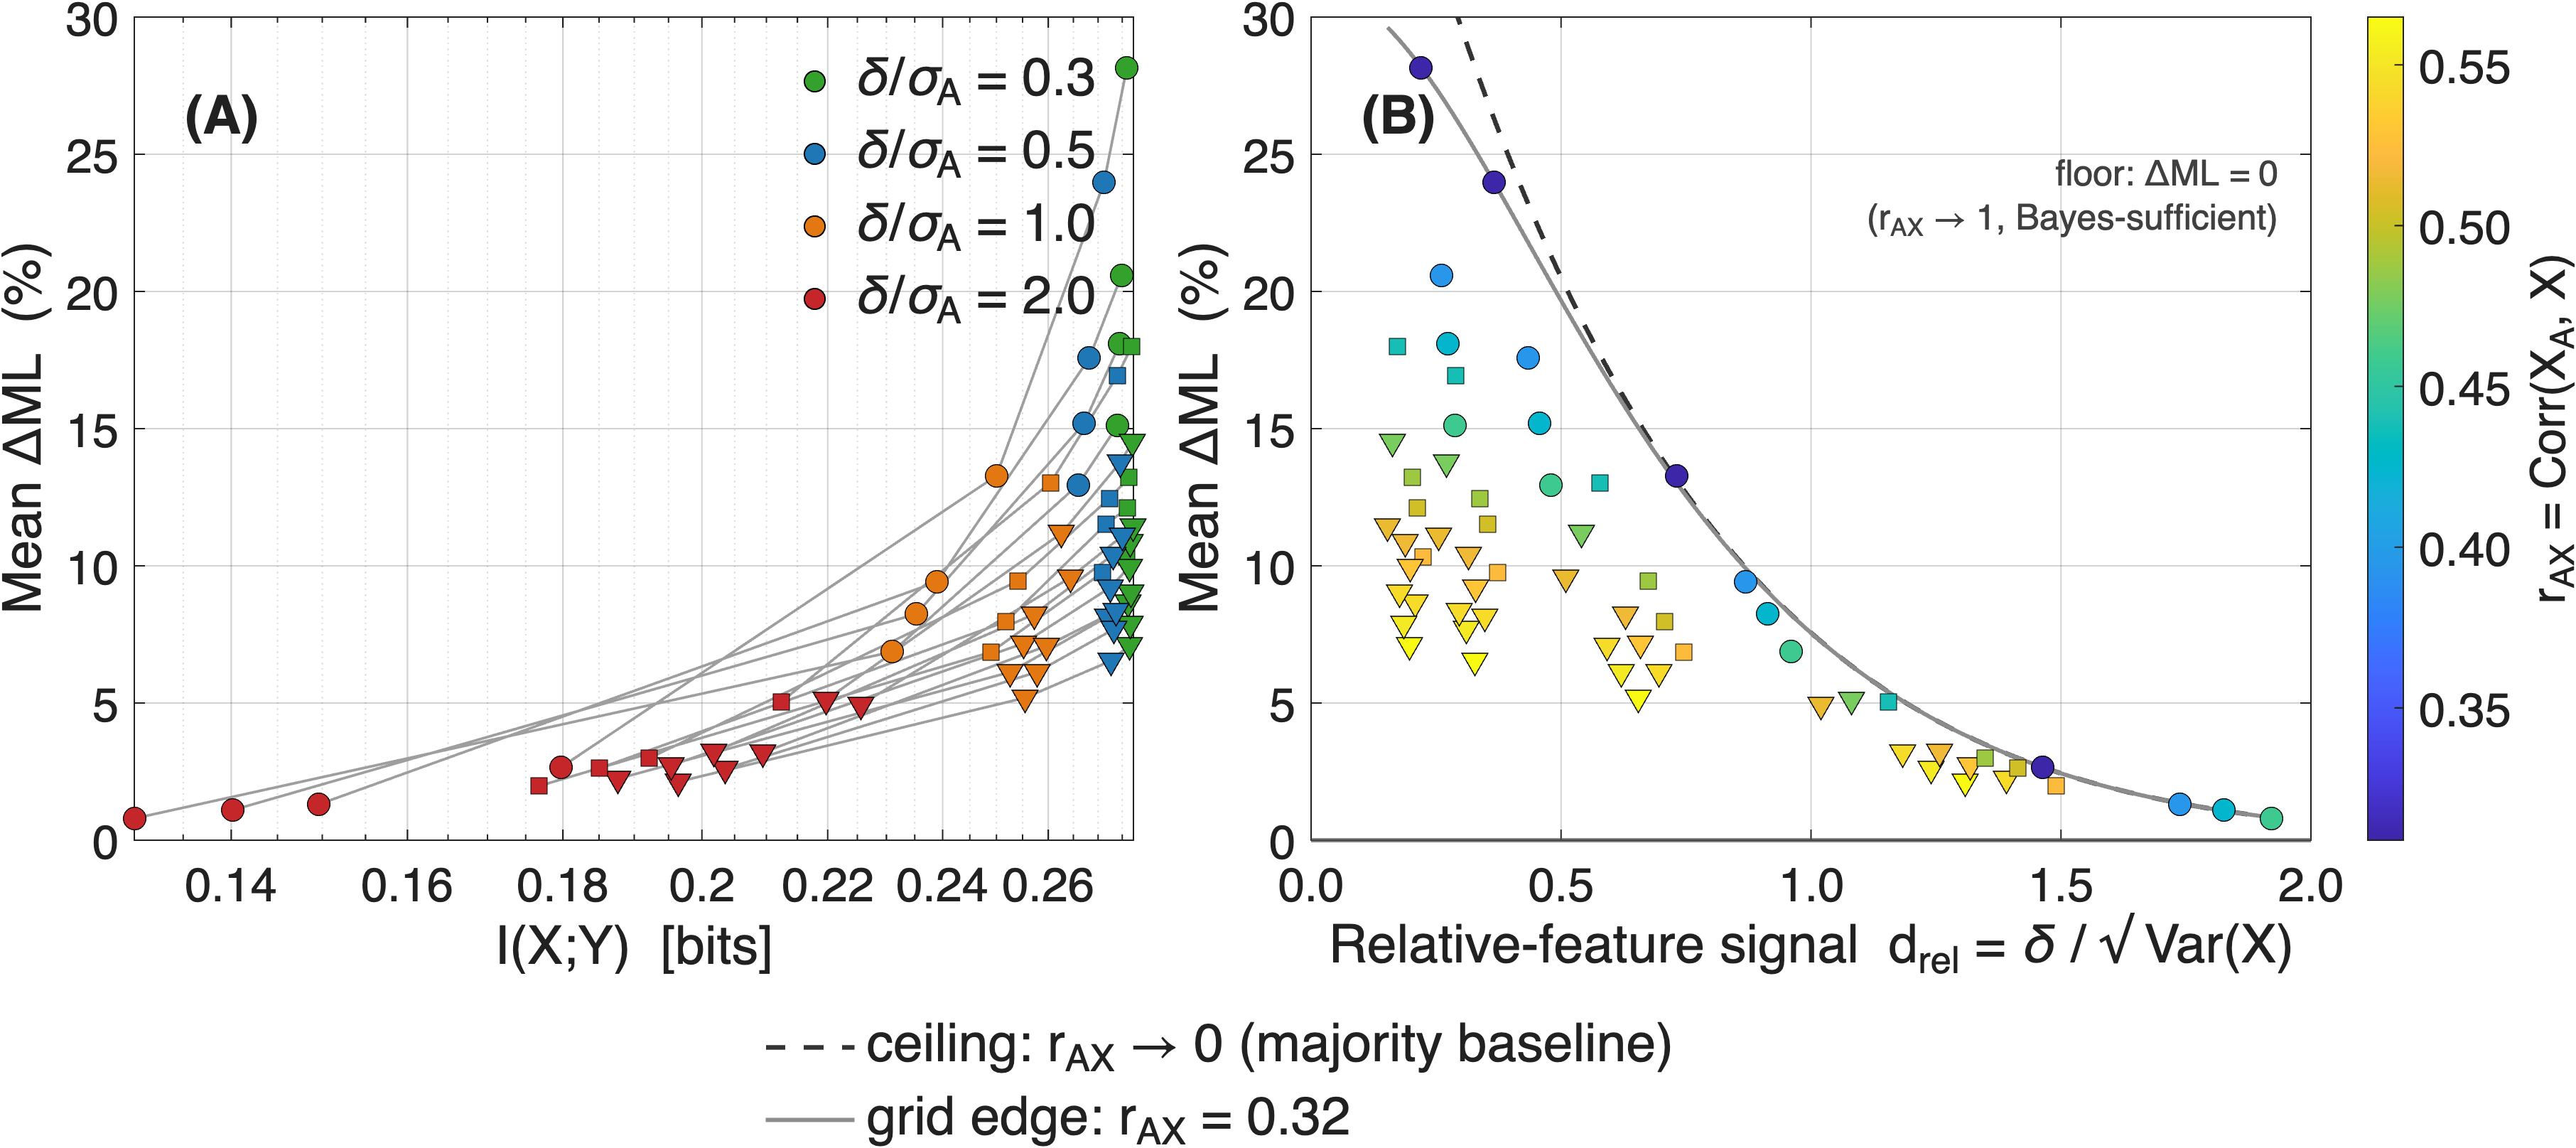
\includegraphics[width=\linewidth]{figures/Figure_S1_idealised_I_vs_dML_overlay.png}
  \caption{Idealised probit simulation (\cref{sec:si_probit}) under (A1)--(A2).
    Grid: $\kappa\in\{0.8,1.0,1.2,2.0\}$, $\rho\in\{-0.3,-0.15,0,0.4\}$,
    $\delta/\sigma_{\mathrm{A}}\in\{0.3,0.5,1.0,2.0\}$
    (64 cells; $n=5{,}000$, 50 trials, five-fold logistic CV).
    (A)~$I(X;Y)$ versus mean $\Delta\mathrm{ML}$ (logarithmic $x$-axis).
    Colour is signal strength. Grey trajectories join the same $(\kappa,\rho)$ across the
    four $\delta/\sigma_{\mathrm{A}}$ values. The colour bands are signal strata, not PEF regimes.
    (B)~Analytic gain surface $\Delta\mathrm{ML}=F(d_{\mathrm{rel}},r_{AX})$ from \cref{sec:si_probit}
    (Pearson correlation $0.9998$ versus simulated CV). Points are coloured by $r_{AX}=\Corr(X_{\mathrm{A}},X)$.
    The dashed curve is the $r_{AX}\to0$ ceiling; the grey curve is the grid edge at $r_{AX}=0.32$.}
  \label{fig:si_idealised_stratified}
\end{figure}

\clearpage

\begin{figure}[h]
  \centering
  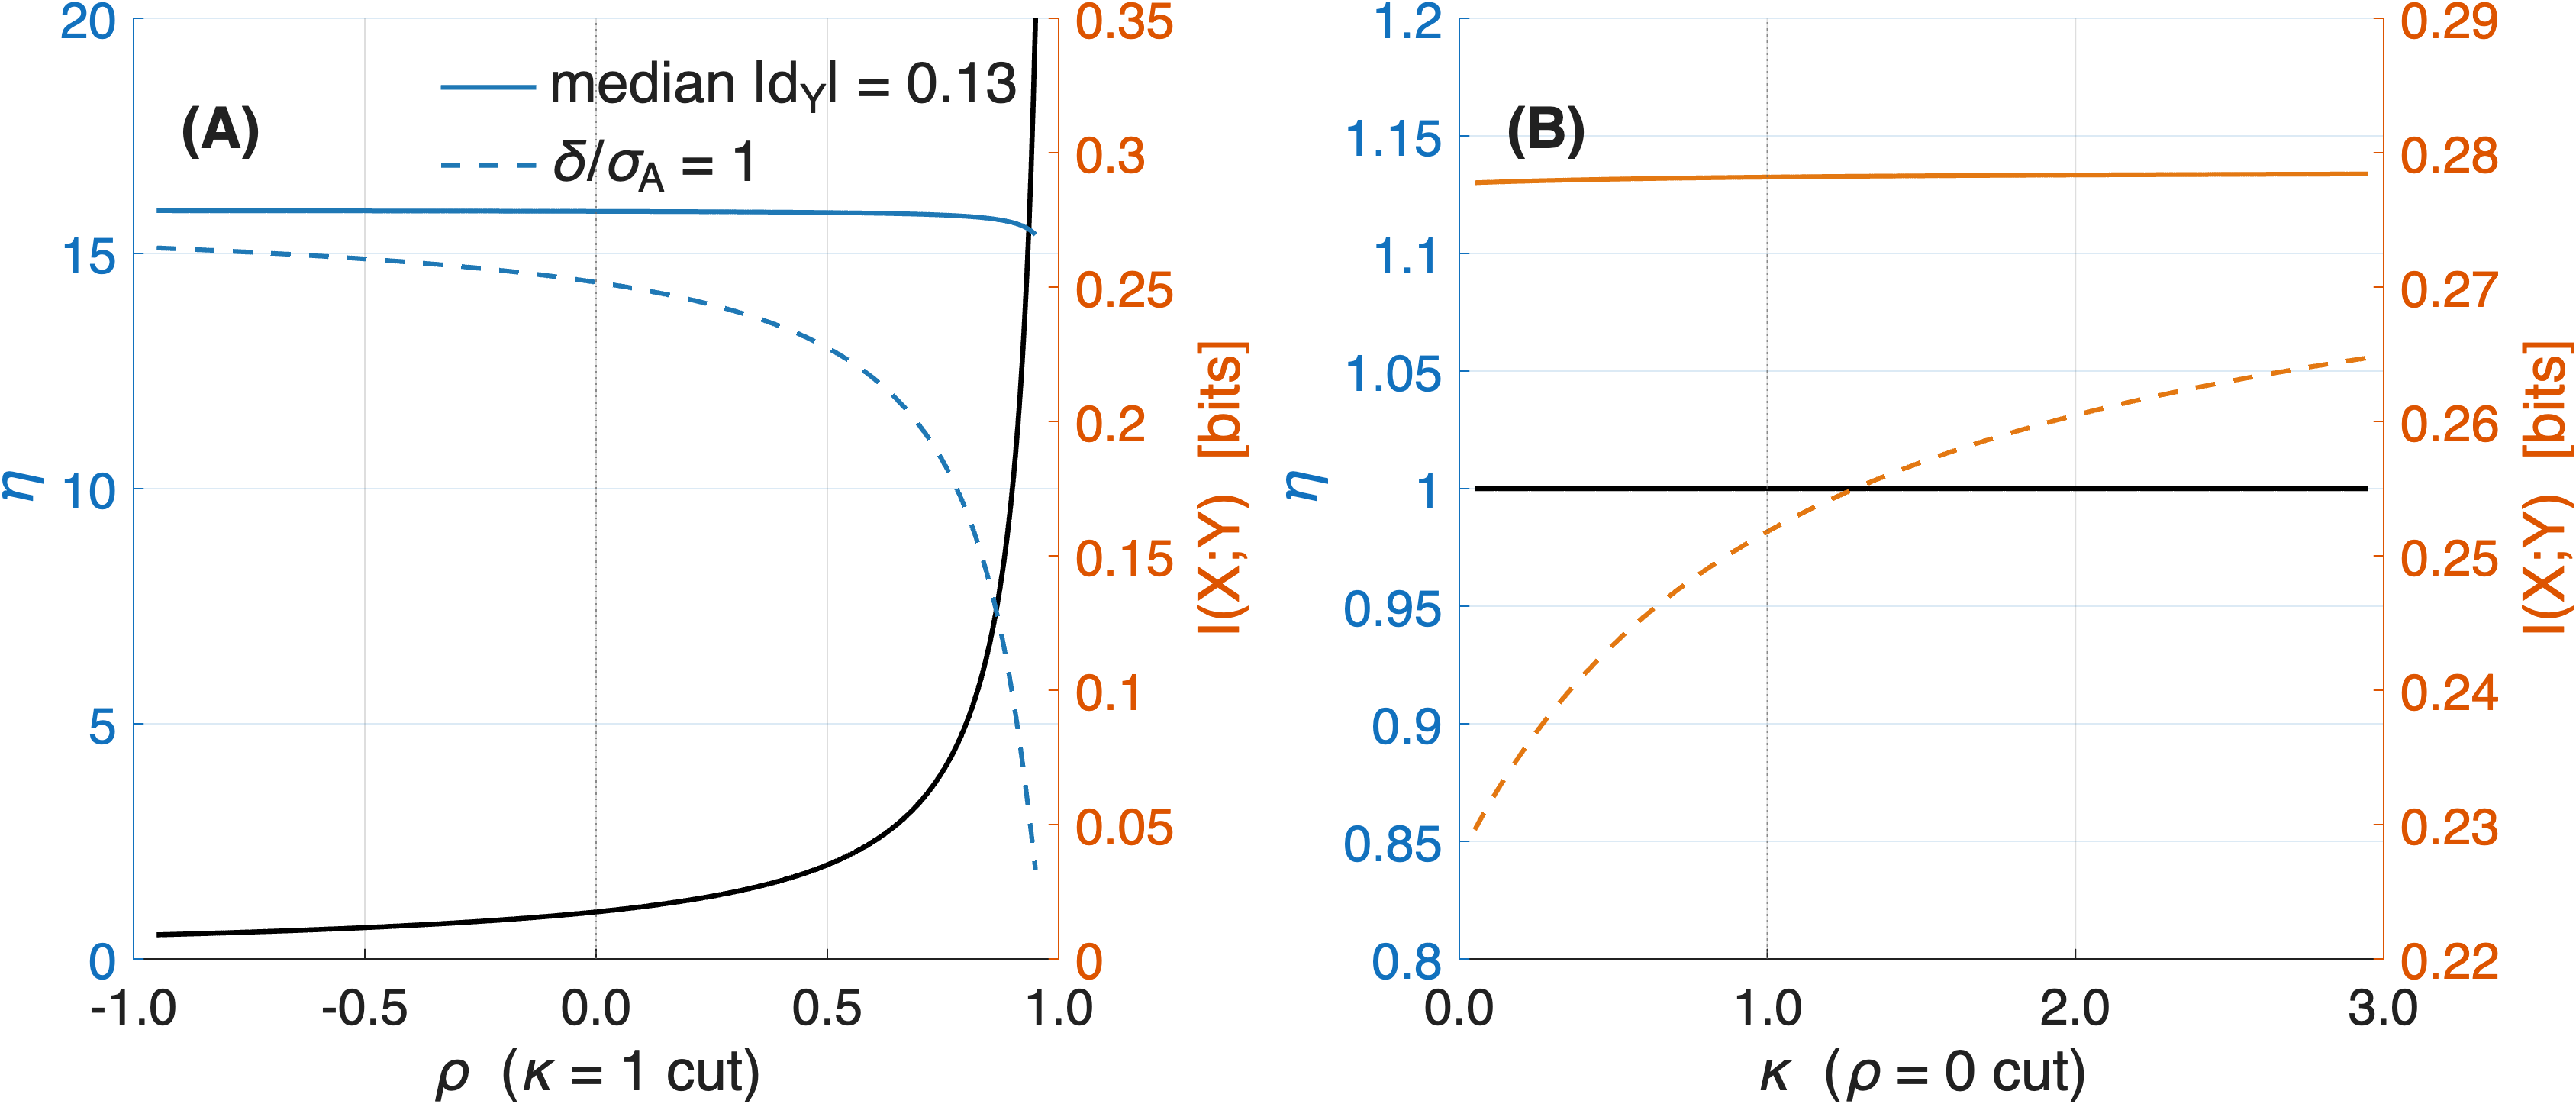
\includegraphics[width=0.85\linewidth]{figures/Figure_S2_iso_eta_I_tension.png}
  \caption{Cuts of $\eta$ and $I(X;Y)$ under the probit model (\cref{sec:si_probit}).
    Solid curves use the median empirical class separation $|\hat d_Y|$.
    Dashed curves use $\delta/\sigma_{\mathrm{A}}=1$.
    The solid curve is not a home--away gap.
    (A)~Cut at $\kappa=1$: $\eta(\rho)$ does not depend on the signal, while $I(\rho)$ is lower at
    $\delta/\sigma_{\mathrm{A}}=1$ than at the median $|\hat d_Y|$, because a larger relative signal makes $Y$ more nearly certain.
    (B)~Cut at $\rho=0$: $\eta=1$ for all $\kappa$; again only $I$ moves with the signal, and it falls as the signal rises.}
  \label{fig:si_iso_eta_I}
\end{figure}

\clearpage

% ---------------------------------------------------------------------------
\refstepcounter{sisection}
\section*{SI Section \thesisection: Empirical Analysis}
\label{sec:si_landscape}

\noindent This section supports the descriptive mapping (\cref{sec:outcome_defs,sec:results}) of the $\PEFtotalStudies{}$ rugby and football KPIs. The cloud is \cref{fig:pef_landscape}. This section gives class separation against $\Delta\mathrm{ML}$ (\cref{fig:si_ipred_vs_dml}), quadrant-level aggregates (Table~S1), and quality-control checks. The home--away gap is not plugged into $I(X;Y)$.

\begin{figure}[h]
  \centering
  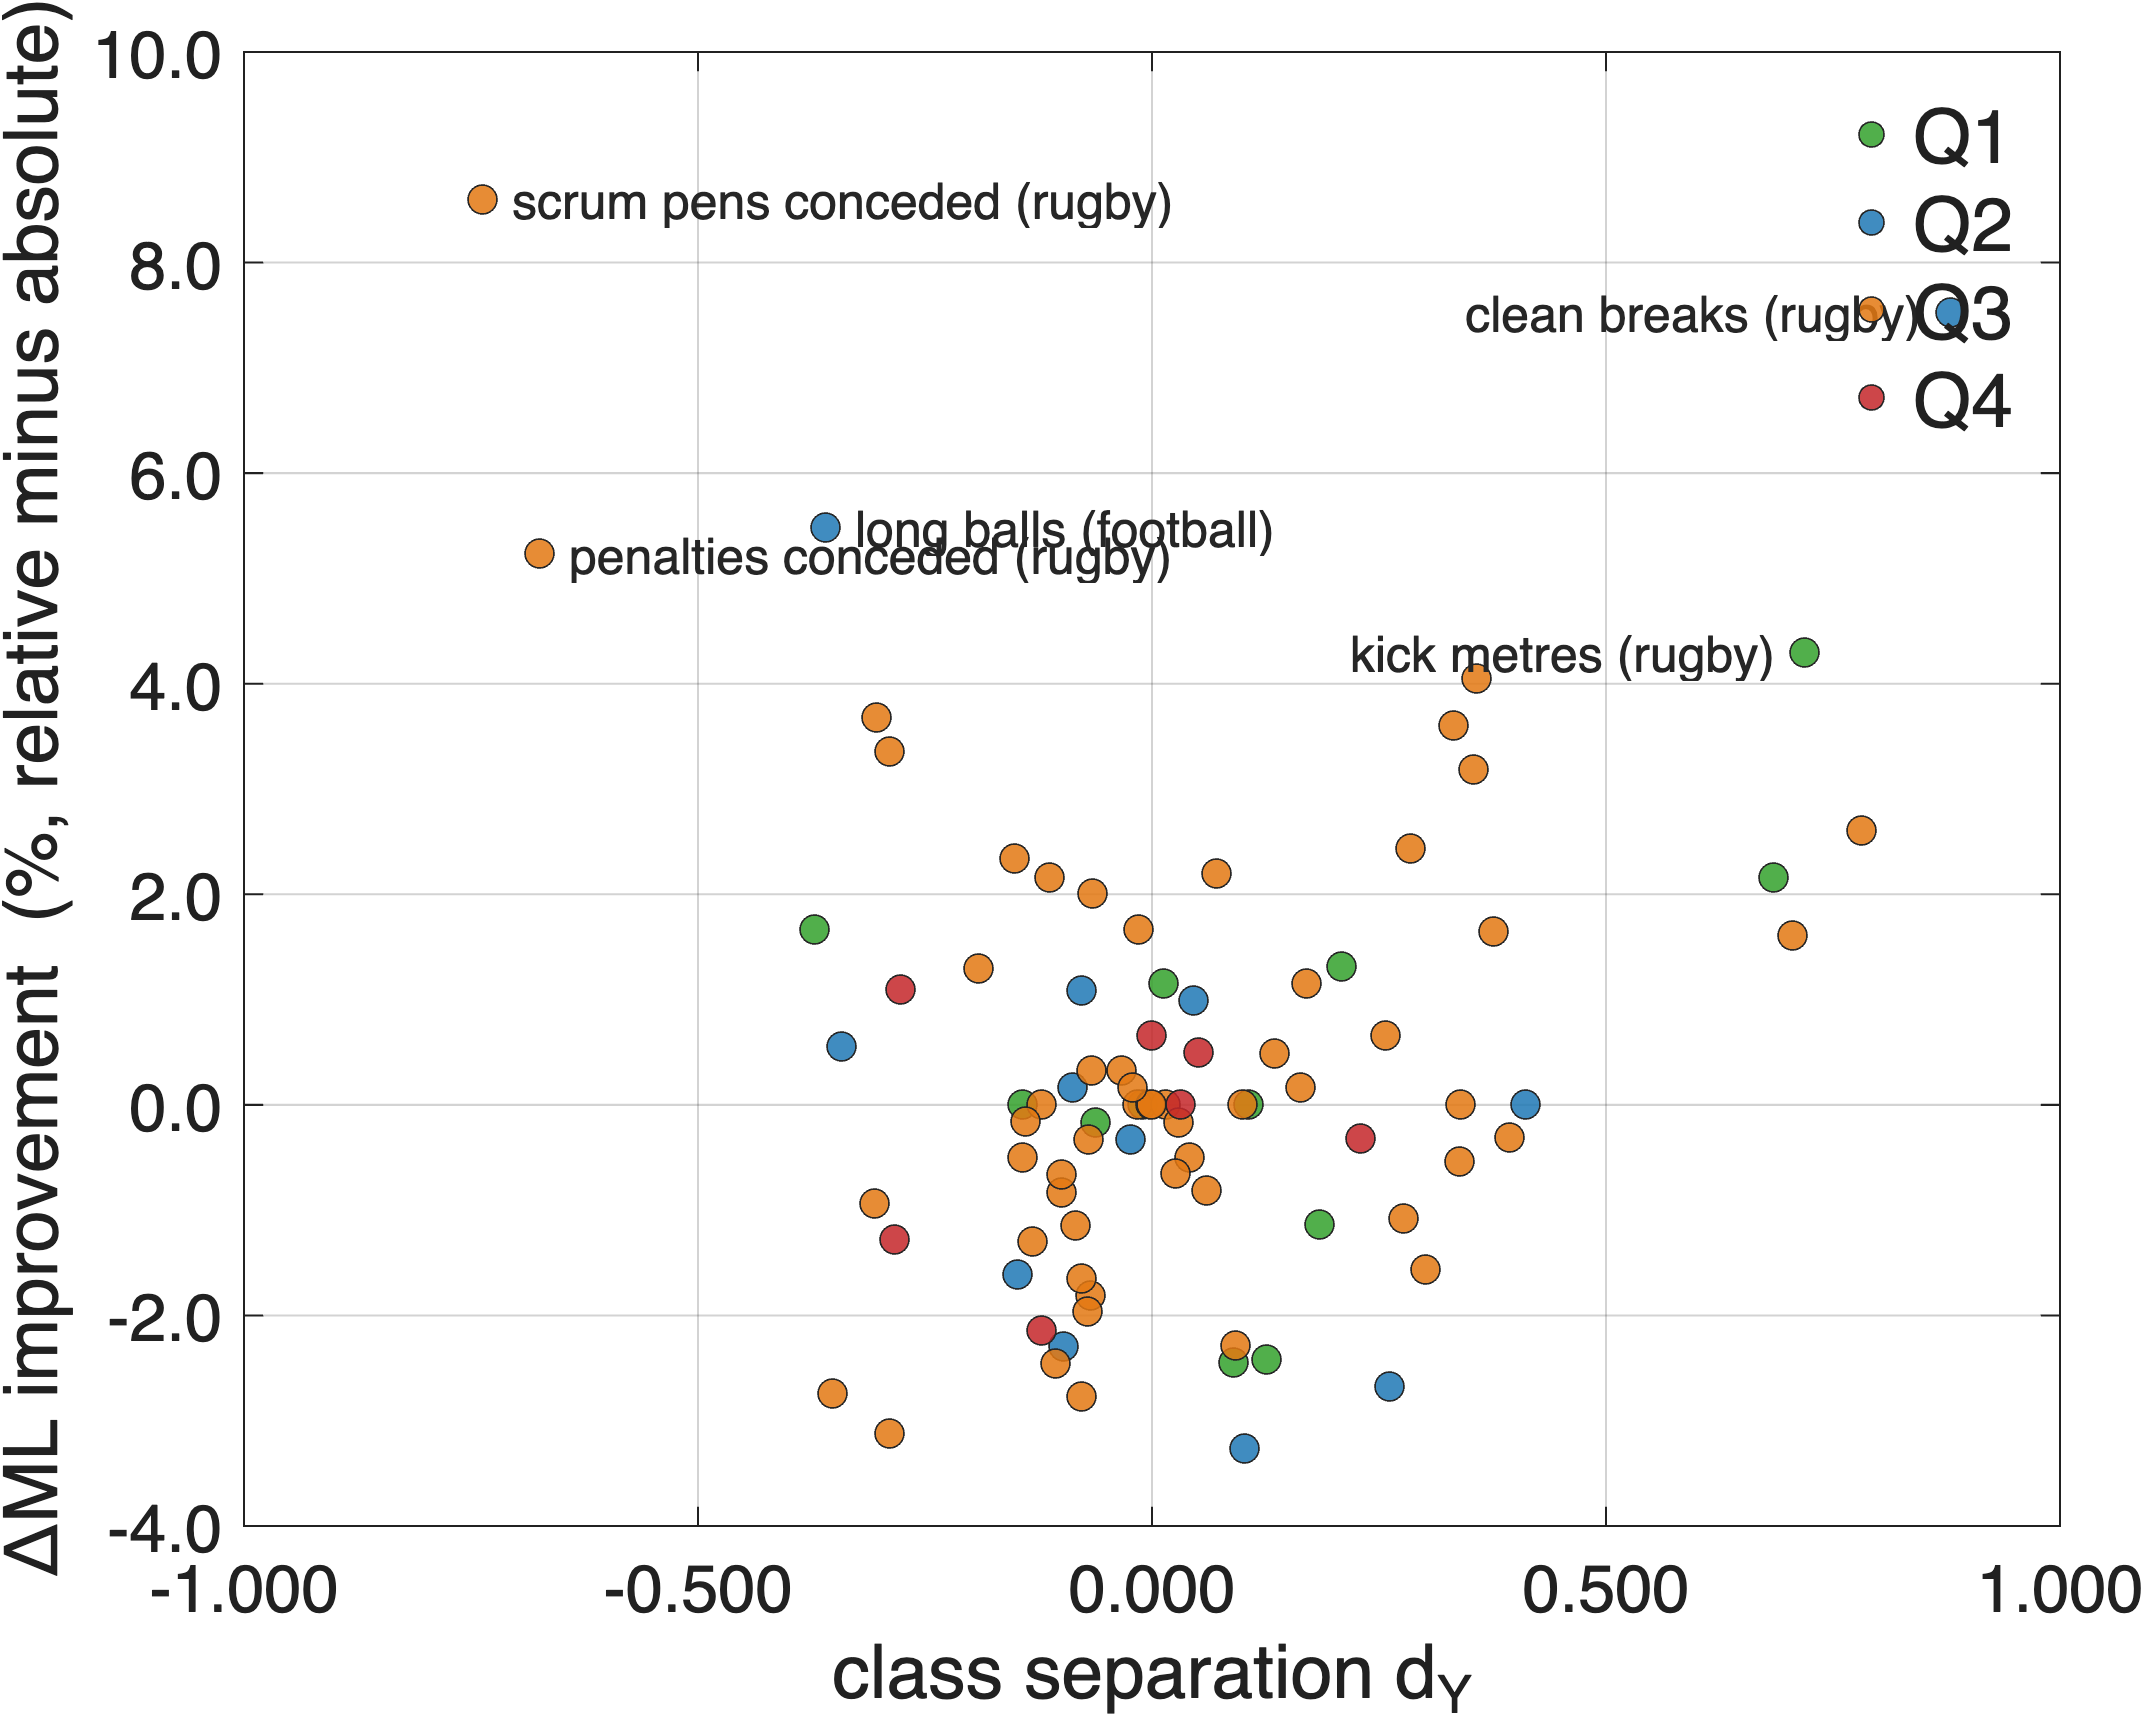
\includegraphics[width=0.85\linewidth]{figures/Figure_S5_Ipred_vs_dML.png}
  \caption{Class separation does not line up with the accuracy change.
    $\hat d_Y$ versus team-blocked five-fold $\Delta\mathrm{ML}$
    across $N=\PEFtotalStudies$ sports KPIs (pooled seasons 23/24--24/25).
    Most of these KPIs lie in Quadrant~3.
    The correlation is $r=\PEFcorrIpredML$ (\cref{sec:outcome_defs}).
    The correlation of $\hat\eta$ with $\Delta\mathrm{ML}$ on the same KPIs is $r=\PEFcorrEtaML$.
    Labelled points are the five largest $|\Delta\mathrm{ML}|$ values among action KPIs.
    The home--away gap is not the horizontal axis.}
  \label{fig:si_ipred_vs_dml}
\end{figure}

\clearpage

\begin{table}[h]
  \centering
  \caption{Descriptive quadrant-level statistics across the rugby and football KPIs (seasons 23/24--24/25 pooled).}
  \label{tab:si_quad_landscape}
  \begin{tabular}{@{}lccccc@{}}
    \toprule
    \textbf{Q} & \textbf{$n$} & \textbf{Mean $\hat\eta$} & \textbf{95\% CI} & \textbf{\% $\hat\eta>1$} & \textbf{Mean $\Delta\mathrm{ML}$} \\
    \midrule
    Q1 & \PEFqOneNkpis   & \PEFqOneMeanEta   & $[\PEFqOneCIlo,\PEFqOneCIhi]$     & 100 & \PEFqOneMLimpr\% \\
    Q2 & \PEFqTwoNkpis   & \PEFqTwoMeanEta   & $[\PEFqTwoCIlo,\PEFqTwoCIhi]$     & 100 & \PEFqTwoMLimpr\% \\
    Q3 & \PEFqThreeNkpis & \PEFqThreeMeanEta & $[\PEFqThreeCIlo,\PEFqThreeCIhi]$ & 0   & \PEFqThreeMLimpr\% \\
    Q4 & \PEFqFourNkpis  & \PEFqFourMeanEta  & $[\PEFqFourCIlo,\PEFqFourCIhi]$   & 0   & \PEFqFourMLimpr\% \\
    \bottomrule
  \end{tabular}

  \medskip
  \begin{minipage}{0.95\linewidth}\small
    Mean $\Delta\mathrm{ML}$: team-blocked five-fold cross-validated accuracy improvement (relative minus absolute features), pooled across KPIs in the quadrant (\cref{sec:ml_cv}). 95\% CIs are $\pm1.96$ standard errors of the within-quadrant mean $\hat\eta$. Descriptive mapping only; confirmatory checks use \cref{tab:exemplars}. It is not a recommendation to relativise generic Q3 KPIs.
  \end{minipage}
\end{table}

\subsection*{Quality control}
\label{sec:si_qc}

\noindent This subsection supports normality and transformation checks in Methods (\cref{sec:qc}) and distributional limitations in Discussion.

\subsubsection*{Paired-difference normality}
\label{sec:si_normality}

The information-content mapping (\cref{eq:mi_closed}) uses assumption (A1) on the pair $(X_{\mathrm{A}},X_{\mathrm{B}})$. The relevant check for that approximation is the per-match paired difference $X=X_{\mathrm{A}}-X_{\mathrm{B}}$, not the separate home or away series. On the two-season primary window the difference series rejects normality for $\PEFrugbySwReject\%$ of rugby KPIs and $\PEFfootSwReject\%$ of football KPIs. Mean Shapiro--Wilk $W$ is $0.977$ in rugby and $0.986$ in football, with mean skewness $0.028$ and $0.069$ (\texttt{normality\_commentary.csv}). Home and away series are more right-skewed, as expected for count KPIs. Low-count discrete KPIs can reject for that reason. The PEF formula itself does not require normality.

\subsubsection*{Log-transform and Quadrant~4 bootstrap}
\label{sec:si_landscape_qc}
\label{sec:si_note_s1}

A log-transform $Z=\log(X+1)$ on the \PEFrugbyNkpis{} rugby action KPIs preserves rank order by $\rho$ (Spearman $r_{s}=0.967$; mean $|\rho_{\log}-\rho|=0.032$). The mean of the KPI-wise ratios $\eta_{\log}/\eta$ is $1.085$ (median $1.002$; paired $t$, $p=0.357$). That mean is pulled by rucks won. The transform is a sensitivity check for right-skewed counts, not a default step.

Team-cluster bootstrap percentile intervals use $B=1{,}000$ home-team resamples (\cref{sec:qc}). For fouls, the confirmatory Quadrant~4 KPI, the interval for $\hat\eta$ is $[0.897, 1.027]$, which includes one (point estimate $\PEFexQfourEta$; \cref{tab:exemplars}). For tackles (rugby, Quadrant~4) the interval is $[0.773, 0.946]$, entirely below one. Away matches of a resampled club can remain in the bootstrap, because the cluster is the home team.

\label{sec:si_practitioner}
\label{sec:si_note_s4}
The open SI2 and SI3 tools for the six-step procedure in \cref{sec:practical_guidance} are documented at \cref{sec:data_availability}.
